% LaTeX snippets generated for individually exported K-debug panels.
% Add this package in the preamble if it is not already present:
% \usepackage[caption=false,font=footnotesize]{subfig}

% ACA-RSA: Fallback success rate
\begin{figure*}[t]
\centering
\subfloat[German]{%
\includegraphics[width=0.32\textwidth]{aca_rsa_fallback_success_rate_GERMAN.pdf}%
}
\subfloat[TI]{%
\includegraphics[width=0.32\textwidth]{aca_rsa_fallback_success_rate_TI.pdf}%
}
\subfloat[USNET]{%
\includegraphics[width=0.32\textwidth]{aca_rsa_fallback_success_rate_USNET.pdf}%
}
\caption{Fallback success rate for ACA-RSA.}
\label{fig:aca_rsa_fallback_success_rate}
\end{figure*}

% ACA-RSA: Average selected path count
\begin{figure*}[t]
\centering
\subfloat[German]{%
\includegraphics[width=0.32\textwidth]{aca_rsa_average_k_selected_GERMAN.pdf}%
}
\subfloat[TI]{%
\includegraphics[width=0.32\textwidth]{aca_rsa_average_k_selected_TI.pdf}%
}
\subfloat[USNET]{%
\includegraphics[width=0.32\textwidth]{aca_rsa_average_k_selected_USNET.pdf}%
}
\caption{Average selected path count for ACA-RSA.}
\label{fig:aca_rsa_average_k_selected}
\end{figure*}

% ACA-RSA: Average effective path count
\begin{figure*}[t]
\centering
\subfloat[German]{%
\includegraphics[width=0.32\textwidth]{aca_rsa_average_k_effective_GERMAN.pdf}%
}
\subfloat[TI]{%
\includegraphics[width=0.32\textwidth]{aca_rsa_average_k_effective_TI.pdf}%
}
\subfloat[USNET]{%
\includegraphics[width=0.32\textwidth]{aca_rsa_average_k_effective_USNET.pdf}%
}
\caption{Average effective path count for ACA-RSA.}
\label{fig:aca_rsa_average_k_effective}
\end{figure*}

% ACA-RSA: Average non-contributing path ratio
\begin{figure*}[t]
\centering
\subfloat[German]{%
\includegraphics[width=0.32\textwidth]{aca_rsa_average_non_contributing_path_ratio_GERMAN.pdf}%
}
\subfloat[TI]{%
\includegraphics[width=0.32\textwidth]{aca_rsa_average_non_contributing_path_ratio_TI.pdf}%
}
\subfloat[USNET]{%
\includegraphics[width=0.32\textwidth]{aca_rsa_average_non_contributing_path_ratio_USNET.pdf}%
}
\caption{Average non-contributing path ratio for ACA-RSA.}
\label{fig:aca_rsa_average_non_contributing_path_ratio}
\end{figure*}

% ACA-RSA: Average redundancy r
\begin{figure*}[t]
\centering
\subfloat[German]{%
\includegraphics[width=0.32\textwidth]{aca_rsa_average_redundancy_r_GERMAN.pdf}%
}
\subfloat[TI]{%
\includegraphics[width=0.32\textwidth]{aca_rsa_average_redundancy_r_TI.pdf}%
}
\subfloat[USNET]{%
\includegraphics[width=0.32\textwidth]{aca_rsa_average_redundancy_r_USNET.pdf}%
}
\caption{Average redundancy r for ACA-RSA.}
\label{fig:aca_rsa_average_redundancy_r}
\end{figure*}

% ACA-RSA: Selected path count distribution
\begin{figure*}[t]
\centering
\subfloat[German]{%
\includegraphics[width=0.32\textwidth]{aca_rsa_k_selected_distribution_GERMAN.pdf}%
}
\subfloat[TI]{%
\includegraphics[width=0.32\textwidth]{aca_rsa_k_selected_distribution_TI.pdf}%
}
\subfloat[USNET]{%
\includegraphics[width=0.32\textwidth]{aca_rsa_k_selected_distribution_USNET.pdf}%
}
\caption{Selected path count distribution for ACA-RSA.}
\label{fig:aca_rsa_k_selected_distribution}
\end{figure*}

% ACA-RSA: Effective path count distribution
\begin{figure*}[t]
\centering
\subfloat[German]{%
\includegraphics[width=0.32\textwidth]{aca_rsa_k_effective_distribution_GERMAN.pdf}%
}
\subfloat[TI]{%
\includegraphics[width=0.32\textwidth]{aca_rsa_k_effective_distribution_TI.pdf}%
}
\subfloat[USNET]{%
\includegraphics[width=0.32\textwidth]{aca_rsa_k_effective_distribution_USNET.pdf}%
}
\caption{Effective path count distribution for ACA-RSA.}
\label{fig:aca_rsa_k_effective_distribution}
\end{figure*}

% ACA-RSA: Successful effective path count distribution
\begin{figure*}[t]
\centering
\subfloat[German]{%
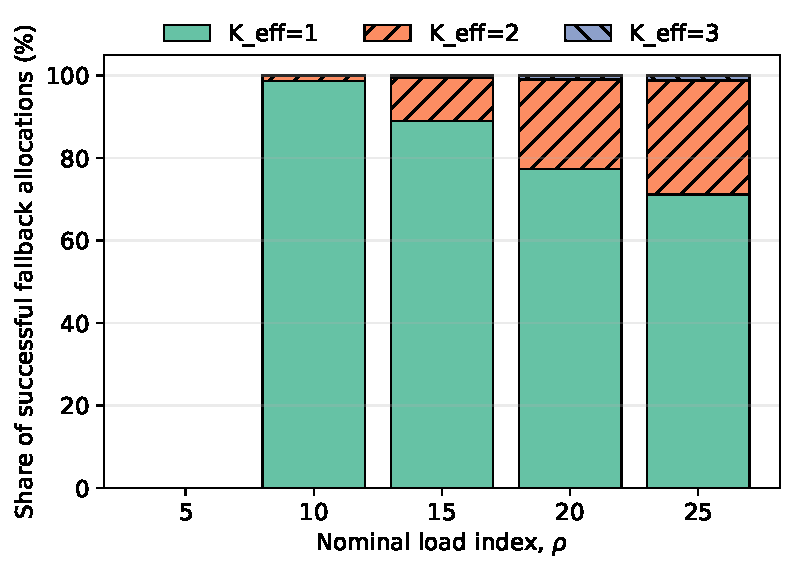
\includegraphics[width=0.32\textwidth]{aca_rsa_k_effective_success_distribution_GERMAN.pdf}%
}
\subfloat[TI]{%
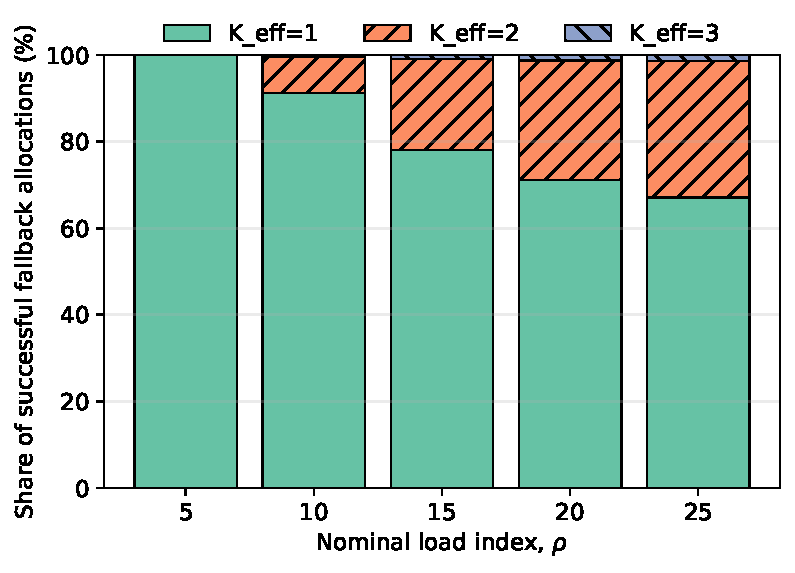
\includegraphics[width=0.32\textwidth]{aca_rsa_k_effective_success_distribution_TI.pdf}%
}
\subfloat[USNET]{%
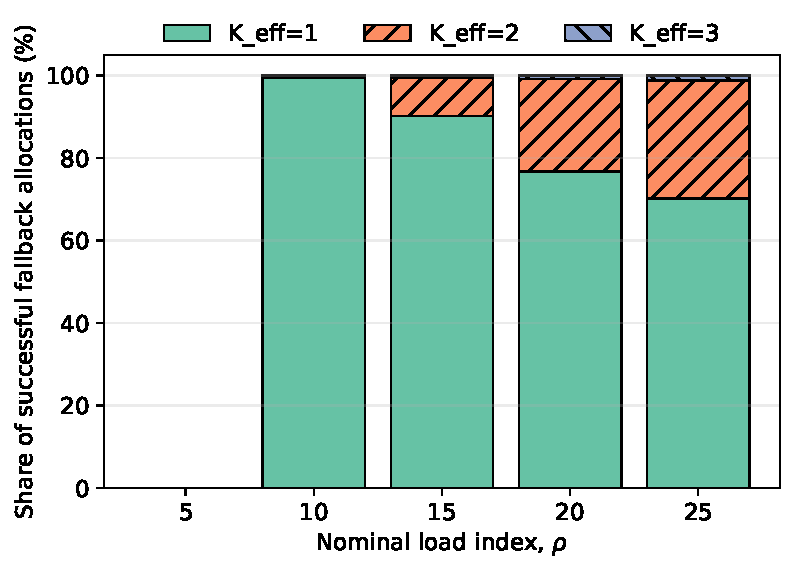
\includegraphics[width=0.32\textwidth]{aca_rsa_k_effective_success_distribution_USNET.pdf}%
}
\caption{Successful effective path count distribution for ACA-RSA.}
\label{fig:aca_rsa_k_effective_success_distribution}
\end{figure*}

% A-MP-SS-RSA: Fallback success rate
\begin{figure*}[t]
\centering
\subfloat[German]{%
\includegraphics[width=0.32\textwidth]{adaptive_mp_ss_rsa_fallback_success_rate_GERMAN.pdf}%
}
\subfloat[TI]{%
\includegraphics[width=0.32\textwidth]{adaptive_mp_ss_rsa_fallback_success_rate_TI.pdf}%
}
\subfloat[USNET]{%
\includegraphics[width=0.32\textwidth]{adaptive_mp_ss_rsa_fallback_success_rate_USNET.pdf}%
}
\caption{Fallback success rate for A-MP-SS-RSA.}
\label{fig:adaptive_mp_ss_rsa_fallback_success_rate}
\end{figure*}

% A-MP-SS-RSA: Average selected path count
\begin{figure*}[t]
\centering
\subfloat[German]{%
\includegraphics[width=0.32\textwidth]{adaptive_mp_ss_rsa_average_k_selected_GERMAN.pdf}%
}
\subfloat[TI]{%
\includegraphics[width=0.32\textwidth]{adaptive_mp_ss_rsa_average_k_selected_TI.pdf}%
}
\subfloat[USNET]{%
\includegraphics[width=0.32\textwidth]{adaptive_mp_ss_rsa_average_k_selected_USNET.pdf}%
}
\caption{Average selected path count for A-MP-SS-RSA.}
\label{fig:adaptive_mp_ss_rsa_average_k_selected}
\end{figure*}

% A-MP-SS-RSA: Average effective path count
\begin{figure*}[t]
\centering
\subfloat[German]{%
\includegraphics[width=0.32\textwidth]{adaptive_mp_ss_rsa_average_k_effective_GERMAN.pdf}%
}
\subfloat[TI]{%
\includegraphics[width=0.32\textwidth]{adaptive_mp_ss_rsa_average_k_effective_TI.pdf}%
}
\subfloat[USNET]{%
\includegraphics[width=0.32\textwidth]{adaptive_mp_ss_rsa_average_k_effective_USNET.pdf}%
}
\caption{Average effective path count for A-MP-SS-RSA.}
\label{fig:adaptive_mp_ss_rsa_average_k_effective}
\end{figure*}

% A-MP-SS-RSA: Average non-contributing path ratio
\begin{figure*}[t]
\centering
\subfloat[German]{%
\includegraphics[width=0.32\textwidth]{adaptive_mp_ss_rsa_average_non_contributing_path_ratio_GERMAN.pdf}%
}
\subfloat[TI]{%
\includegraphics[width=0.32\textwidth]{adaptive_mp_ss_rsa_average_non_contributing_path_ratio_TI.pdf}%
}
\subfloat[USNET]{%
\includegraphics[width=0.32\textwidth]{adaptive_mp_ss_rsa_average_non_contributing_path_ratio_USNET.pdf}%
}
\caption{Average non-contributing path ratio for A-MP-SS-RSA.}
\label{fig:adaptive_mp_ss_rsa_average_non_contributing_path_ratio}
\end{figure*}

% A-MP-SS-RSA: Average redundancy r
\begin{figure*}[t]
\centering
\subfloat[German]{%
\includegraphics[width=0.32\textwidth]{adaptive_mp_ss_rsa_average_redundancy_r_GERMAN.pdf}%
}
\subfloat[TI]{%
\includegraphics[width=0.32\textwidth]{adaptive_mp_ss_rsa_average_redundancy_r_TI.pdf}%
}
\subfloat[USNET]{%
\includegraphics[width=0.32\textwidth]{adaptive_mp_ss_rsa_average_redundancy_r_USNET.pdf}%
}
\caption{Average redundancy r for A-MP-SS-RSA.}
\label{fig:adaptive_mp_ss_rsa_average_redundancy_r}
\end{figure*}

% A-MP-SS-RSA: Selected path count distribution
\begin{figure*}[t]
\centering
\subfloat[German]{%
\includegraphics[width=0.32\textwidth]{adaptive_mp_ss_rsa_k_selected_distribution_GERMAN.pdf}%
}
\subfloat[TI]{%
\includegraphics[width=0.32\textwidth]{adaptive_mp_ss_rsa_k_selected_distribution_TI.pdf}%
}
\subfloat[USNET]{%
\includegraphics[width=0.32\textwidth]{adaptive_mp_ss_rsa_k_selected_distribution_USNET.pdf}%
}
\caption{Selected path count distribution for A-MP-SS-RSA.}
\label{fig:adaptive_mp_ss_rsa_k_selected_distribution}
\end{figure*}

% A-MP-SS-RSA: Effective path count distribution
\begin{figure*}[t]
\centering
\subfloat[German]{%
\includegraphics[width=0.32\textwidth]{adaptive_mp_ss_rsa_k_effective_distribution_GERMAN.pdf}%
}
\subfloat[TI]{%
\includegraphics[width=0.32\textwidth]{adaptive_mp_ss_rsa_k_effective_distribution_TI.pdf}%
}
\subfloat[USNET]{%
\includegraphics[width=0.32\textwidth]{adaptive_mp_ss_rsa_k_effective_distribution_USNET.pdf}%
}
\caption{Effective path count distribution for A-MP-SS-RSA.}
\label{fig:adaptive_mp_ss_rsa_k_effective_distribution}
\end{figure*}

% A-MP-SS-RSA: Successful effective path count distribution
\begin{figure*}[t]
\centering
\subfloat[German]{%
\includegraphics[width=0.32\textwidth]{adaptive_mp_ss_rsa_k_effective_success_distribution_GERMAN.pdf}%
}
\subfloat[TI]{%
\includegraphics[width=0.32\textwidth]{adaptive_mp_ss_rsa_k_effective_success_distribution_TI.pdf}%
}
\subfloat[USNET]{%
\includegraphics[width=0.32\textwidth]{adaptive_mp_ss_rsa_k_effective_success_distribution_USNET.pdf}%
}
\caption{Successful effective path count distribution for A-MP-SS-RSA.}
\label{fig:adaptive_mp_ss_rsa_k_effective_success_distribution}
\end{figure*}

% P-ACA-RSA: Fallback success rate
\begin{figure*}[t]
\centering
\subfloat[German]{%
\includegraphics[width=0.32\textwidth]{p_aca_rsa_fallback_success_rate_GERMAN.pdf}%
}
\subfloat[TI]{%
\includegraphics[width=0.32\textwidth]{p_aca_rsa_fallback_success_rate_TI.pdf}%
}
\subfloat[USNET]{%
\includegraphics[width=0.32\textwidth]{p_aca_rsa_fallback_success_rate_USNET.pdf}%
}
\caption{Fallback success rate for P-ACA-RSA.}
\label{fig:p_aca_rsa_fallback_success_rate}
\end{figure*}

% P-ACA-RSA: Average selected path count
\begin{figure*}[t]
\centering
\subfloat[German]{%
\includegraphics[width=0.32\textwidth]{p_aca_rsa_average_k_selected_GERMAN.pdf}%
}
\subfloat[TI]{%
\includegraphics[width=0.32\textwidth]{p_aca_rsa_average_k_selected_TI.pdf}%
}
\subfloat[USNET]{%
\includegraphics[width=0.32\textwidth]{p_aca_rsa_average_k_selected_USNET.pdf}%
}
\caption{Average selected path count for P-ACA-RSA.}
\label{fig:p_aca_rsa_average_k_selected}
\end{figure*}

% P-ACA-RSA: Average effective path count
\begin{figure*}[t]
\centering
\subfloat[German]{%
\includegraphics[width=0.32\textwidth]{p_aca_rsa_average_k_effective_GERMAN.pdf}%
}
\subfloat[TI]{%
\includegraphics[width=0.32\textwidth]{p_aca_rsa_average_k_effective_TI.pdf}%
}
\subfloat[USNET]{%
\includegraphics[width=0.32\textwidth]{p_aca_rsa_average_k_effective_USNET.pdf}%
}
\caption{Average effective path count for P-ACA-RSA.}
\label{fig:p_aca_rsa_average_k_effective}
\end{figure*}

% P-ACA-RSA: Average non-contributing path ratio
\begin{figure*}[t]
\centering
\subfloat[German]{%
\includegraphics[width=0.32\textwidth]{p_aca_rsa_average_non_contributing_path_ratio_GERMAN.pdf}%
}
\subfloat[TI]{%
\includegraphics[width=0.32\textwidth]{p_aca_rsa_average_non_contributing_path_ratio_TI.pdf}%
}
\subfloat[USNET]{%
\includegraphics[width=0.32\textwidth]{p_aca_rsa_average_non_contributing_path_ratio_USNET.pdf}%
}
\caption{Average non-contributing path ratio for P-ACA-RSA.}
\label{fig:p_aca_rsa_average_non_contributing_path_ratio}
\end{figure*}

% P-ACA-RSA: Average redundancy r
\begin{figure*}[t]
\centering
\subfloat[German]{%
\includegraphics[width=0.32\textwidth]{p_aca_rsa_average_redundancy_r_GERMAN.pdf}%
}
\subfloat[TI]{%
\includegraphics[width=0.32\textwidth]{p_aca_rsa_average_redundancy_r_TI.pdf}%
}
\subfloat[USNET]{%
\includegraphics[width=0.32\textwidth]{p_aca_rsa_average_redundancy_r_USNET.pdf}%
}
\caption{Average redundancy r for P-ACA-RSA.}
\label{fig:p_aca_rsa_average_redundancy_r}
\end{figure*}

% P-ACA-RSA: Selected path count distribution
\begin{figure*}[t]
\centering
\subfloat[German]{%
\includegraphics[width=0.32\textwidth]{p_aca_rsa_k_selected_distribution_GERMAN.pdf}%
}
\subfloat[TI]{%
\includegraphics[width=0.32\textwidth]{p_aca_rsa_k_selected_distribution_TI.pdf}%
}
\subfloat[USNET]{%
\includegraphics[width=0.32\textwidth]{p_aca_rsa_k_selected_distribution_USNET.pdf}%
}
\caption{Selected path count distribution for P-ACA-RSA.}
\label{fig:p_aca_rsa_k_selected_distribution}
\end{figure*}

% P-ACA-RSA: Effective path count distribution
\begin{figure*}[t]
\centering
\subfloat[German]{%
\includegraphics[width=0.32\textwidth]{p_aca_rsa_k_effective_distribution_GERMAN.pdf}%
}
\subfloat[TI]{%
\includegraphics[width=0.32\textwidth]{p_aca_rsa_k_effective_distribution_TI.pdf}%
}
\subfloat[USNET]{%
\includegraphics[width=0.32\textwidth]{p_aca_rsa_k_effective_distribution_USNET.pdf}%
}
\caption{Effective path count distribution for P-ACA-RSA.}
\label{fig:p_aca_rsa_k_effective_distribution}
\end{figure*}

% P-ACA-RSA: Successful effective path count distribution
\begin{figure*}[t]
\centering
\subfloat[German]{%
\includegraphics[width=0.32\textwidth]{p_aca_rsa_k_effective_success_distribution_GERMAN.pdf}%
}
\subfloat[TI]{%
\includegraphics[width=0.32\textwidth]{p_aca_rsa_k_effective_success_distribution_TI.pdf}%
}
\subfloat[USNET]{%
\includegraphics[width=0.32\textwidth]{p_aca_rsa_k_effective_success_distribution_USNET.pdf}%
}
\caption{Successful effective path count distribution for P-ACA-RSA.}
\label{fig:p_aca_rsa_k_effective_success_distribution}
\end{figure*}
